\begin{appendices}
%\section*{Bijlage A}
%\addcontentsline{toc}{section}{Bijlage A}  

\newpage

\begin{landscape}
\section*{OSLO ontology}
\addcontentsline{toc}{section}{OSLO ontology}
\label{appendix:oslo:ontology}
    \begin{figure}[H]
    \centering
    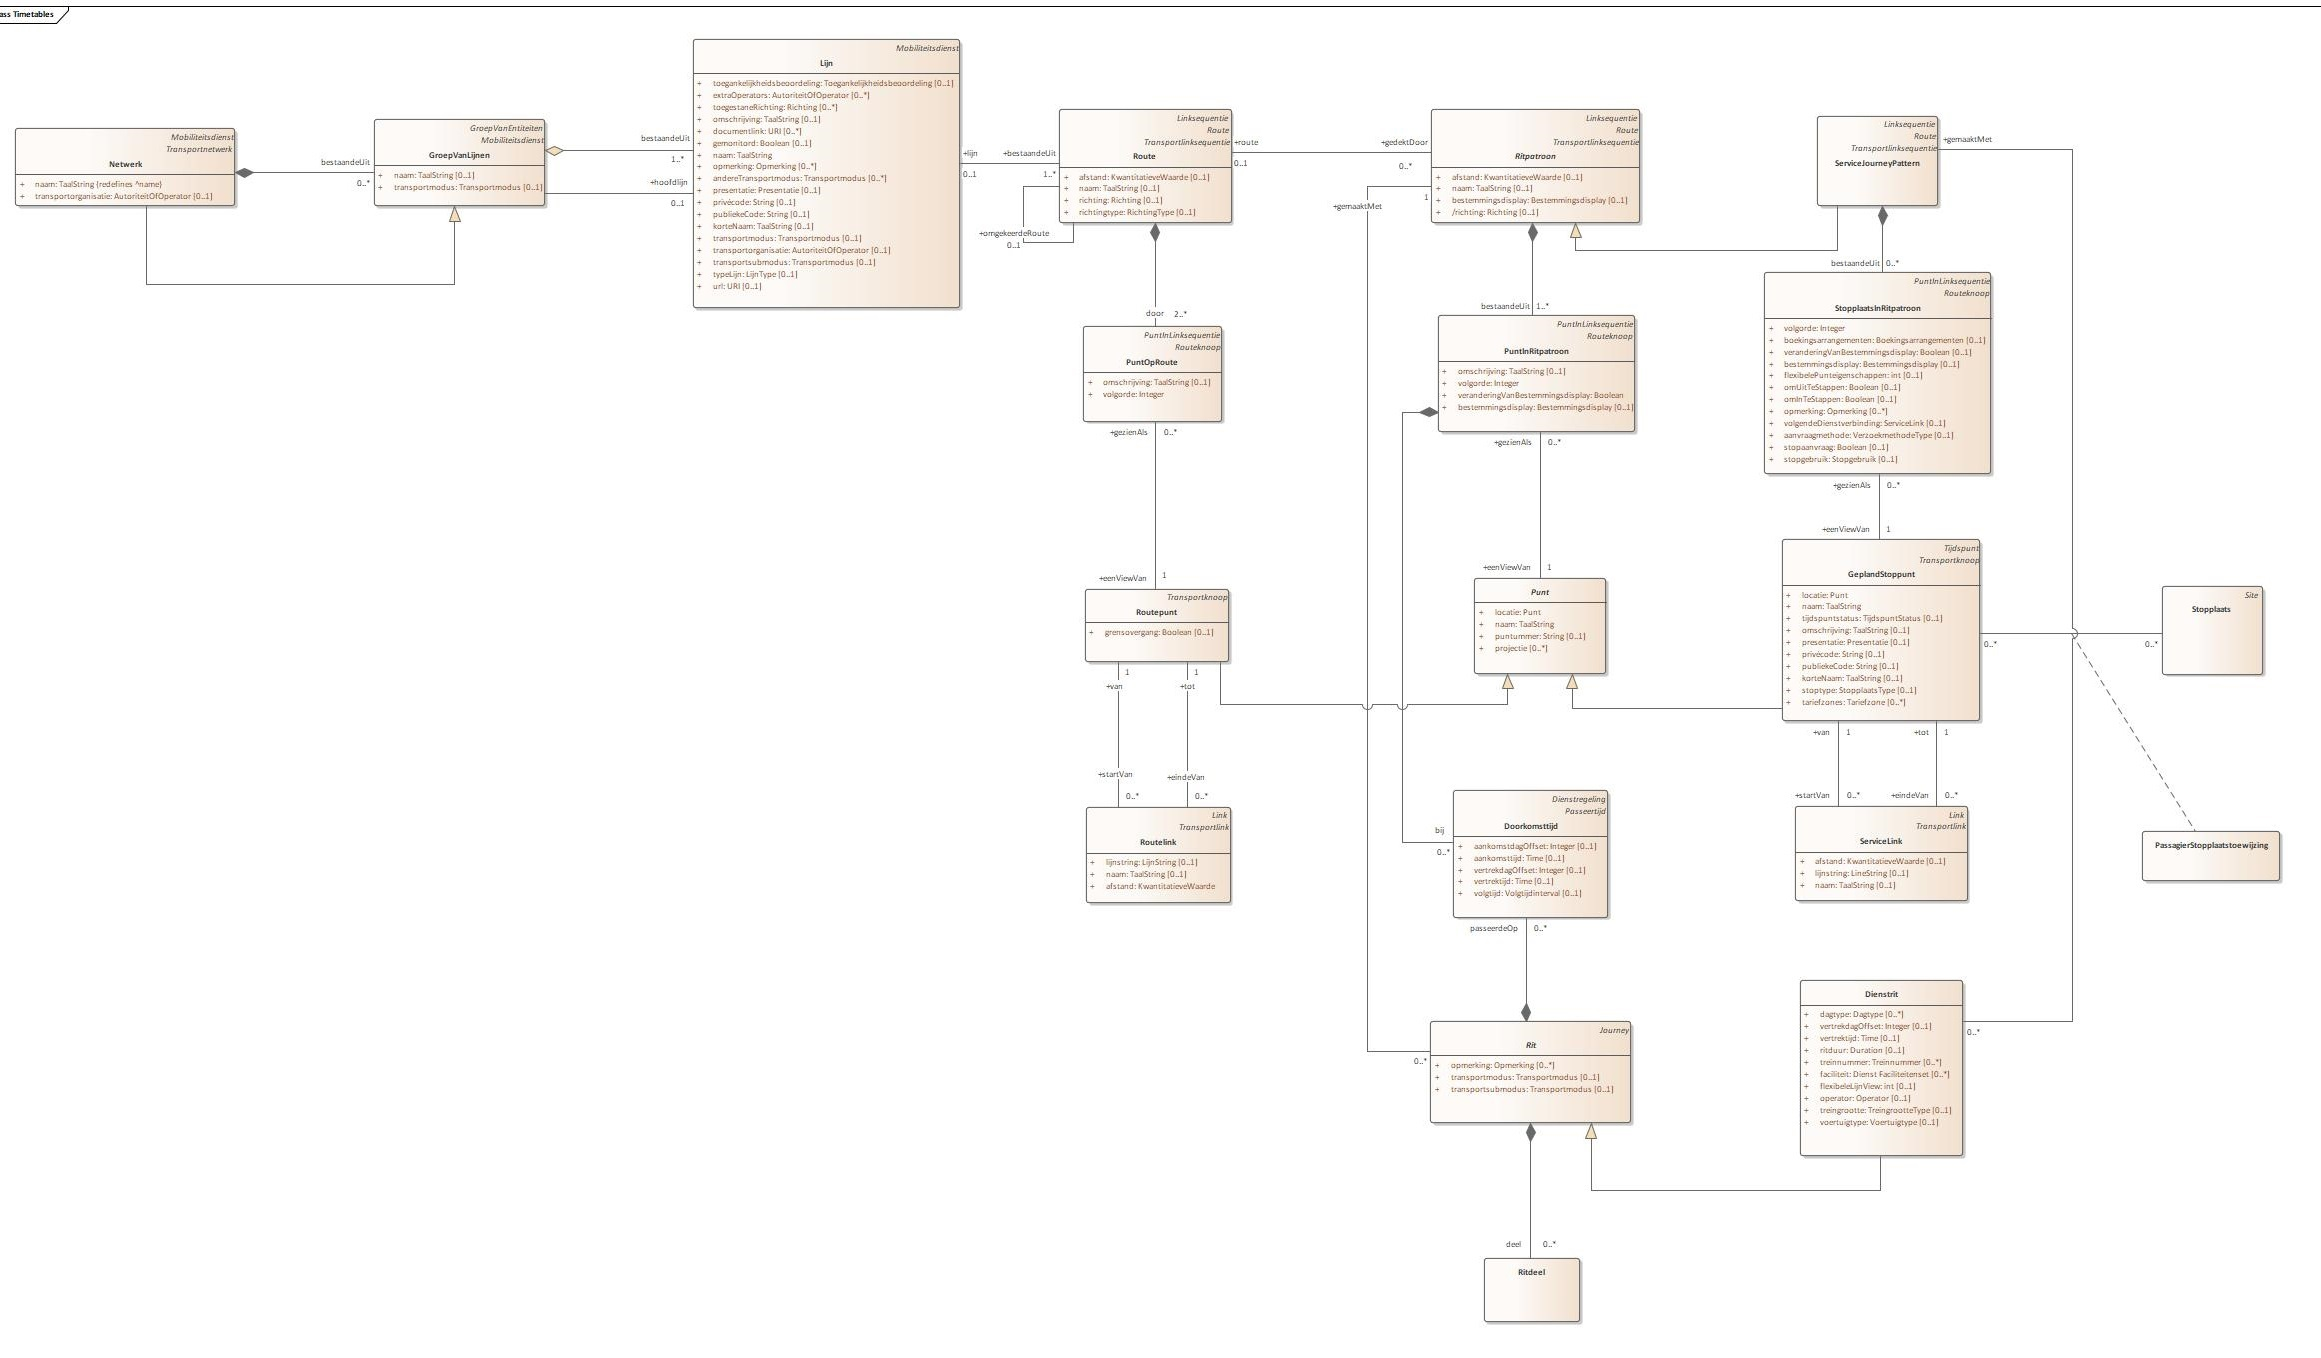
\includegraphics[width=1.4\textwidth]{images/overview.jpg}
    \caption{A small overview of the most important classes in the OSLO Mobility: timetable and route planning algorithm. }
    \tiny For a complete overview, go to \url{https://data.vlaanderen.be/doc/applicatieprofiel/mobiliteit/dienstregeling-en-planning/tijdstabellen/#introduction}
    \label{fig:appendix:Ontology:oslo:overview}
\end{figure}
\end{landscape}

\begin{landscape}
    \section*{History of routing algorithms: timeline}
    \addcontentsline{toc}{section}{History of routing algorithms: timeline} 
    \begin{figure}[H]
\centering
\resizebox{1.7\textwidth}{!}{%
    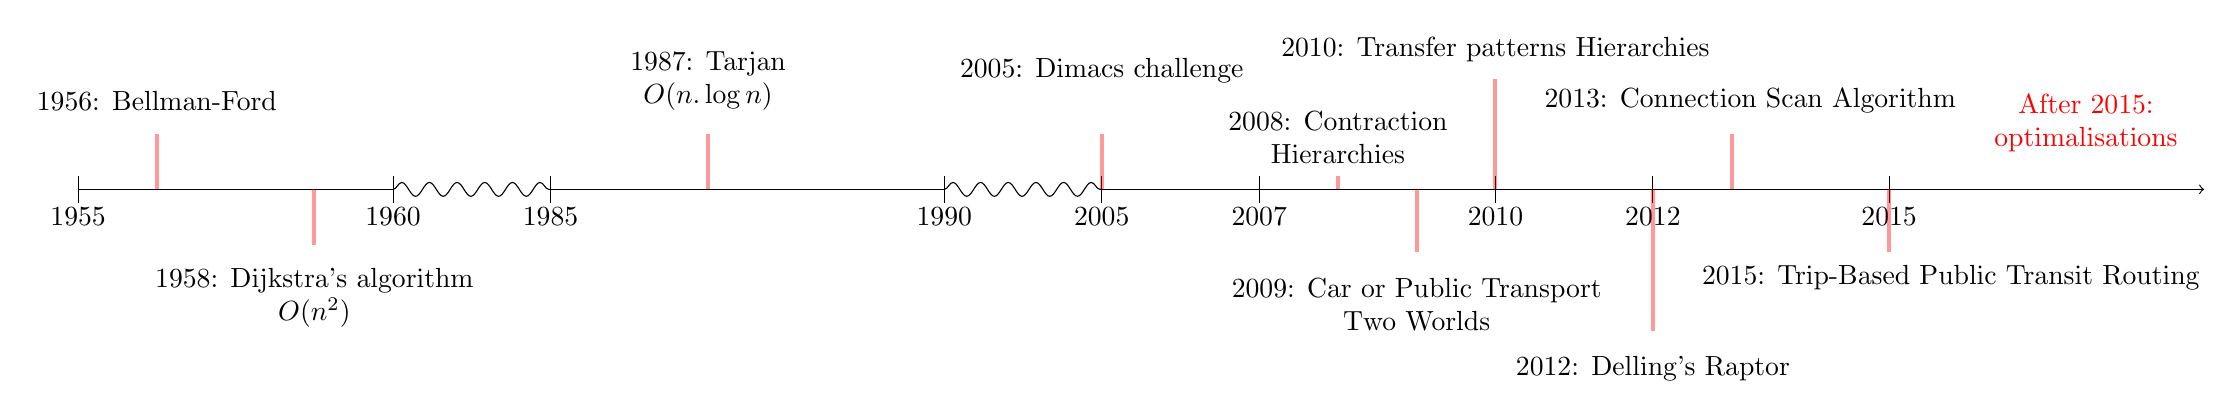
\begin{tikzpicture}
    % Draw a horizontal line
    \draw (0,0) -- (4,0);
    \draw (6,0) -- (11,0);
    \draw (13,0) edge[->] (27,0);
    
    % draw vertical lines
    \foreach \x in {0,4,6,11,13,18,23,15,20}
    \draw (\x cm,5pt) -- (\x cm,-5pt);
    
    \foreach \x in {1,8,13,21}
    \draw[line width=0.5mm, red, opacity=0.4 ] (\x cm,20pt) -- (\x cm,0);
    
    \foreach \x in {3}
    \draw[line width=0.5mm, red, opacity=0.4 ] (\x cm,0) -- (\x cm,-20pt);
    
    % draw nodes to add events
    \draw (0,0) node[below=3pt] {1955};
    \draw (4,0) node[below=3pt] {1960};
    \draw (6,0) node[below=3pt] {1985};
    \draw (11,0) node[below=3pt] {1990};
    \draw (13,0) node[below=3pt] {2005};
    \draw (15,0) node[below=3pt] {2007};
    \draw (18,0) node[below=3pt] {2010};
    \draw (20,0) node[below=3pt] {2012};
    \draw (23,0) node[below=3pt] {2015};

    \draw (25.5,0) node[above=10pt,align=center,text=red] {After 2015:\\ optimalisations};
    
    \draw (1,0) node[above=25pt] {1956: Bellman-Ford};
    
    \draw (3,0) node[below=25pt, align=center] {1958: Dijkstra’s algorithm\\ $O(n^2)$};
    
    \draw (8,0) node[above=25pt, align=center] {1987: Tarjan\\ $O(n.\log{n})$};
    
    \draw (13,0) node[above=35pt] {2005: Dimacs challenge};
    
    \draw (16,0) node[above=0.2cm, align=center] {2008: Contraction \\Hierarchies};
    \draw[line width=0.5mm, red, opacity=0.4 ] (16 cm,5pt) -- (16 cm,0);
    
    \draw (17,0) node[below=1cm, align=center] {2009: Car or Public Transport\\ Two Worlds};
    \draw[line width=0.5mm, red , opacity=0.4] (17 cm,0) -- (17 cm,-0.8cm);
    
    
    \draw (18,0) node[above=1.5cm] {2010: Transfer patterns Hierarchies};
    \draw[line width=0.5mm, red , opacity=0.4] (18 cm,1.4cm) -- (18 cm,0);
    
    \draw (20,0) node[below=2cm] {2012: Delling’s Raptor};
    \draw[line width=0.5mm, red, opacity=0.4] (20 cm,0) -- (20 cm,-1.8cm);
    
    \draw (21,0) node[above=32pt,right=-2.5 cm] {2013: Connection Scan Algorithm};

    \draw (23,0) node[below=32pt,right=-2.5 cm] {2015: Trip-Based Public Transit Routing};
    \draw[line width=0.5mm, red, opacity=0.4] (23 cm,0) -- (23 cm,-0.8cm);
    
    
    \draw[decoration={snake},decorate] (4,0) -- (6,0);
    \draw[decoration={snake},decorate] (11,0) -- (13,0);
    \end{tikzpicture}
    }
    \caption{Timeline describing the developments in route planning. The crossed parts represent}
    \label{fig:timelinelarge}
\end{figure}
\end{landscape}
\section*{Transmodel evolution (first 3 parts)}
\addcontentsline{toc}{section}{Transmodel evolution (first 3 parts)} 
\begin{figure}[H]
    \centering
    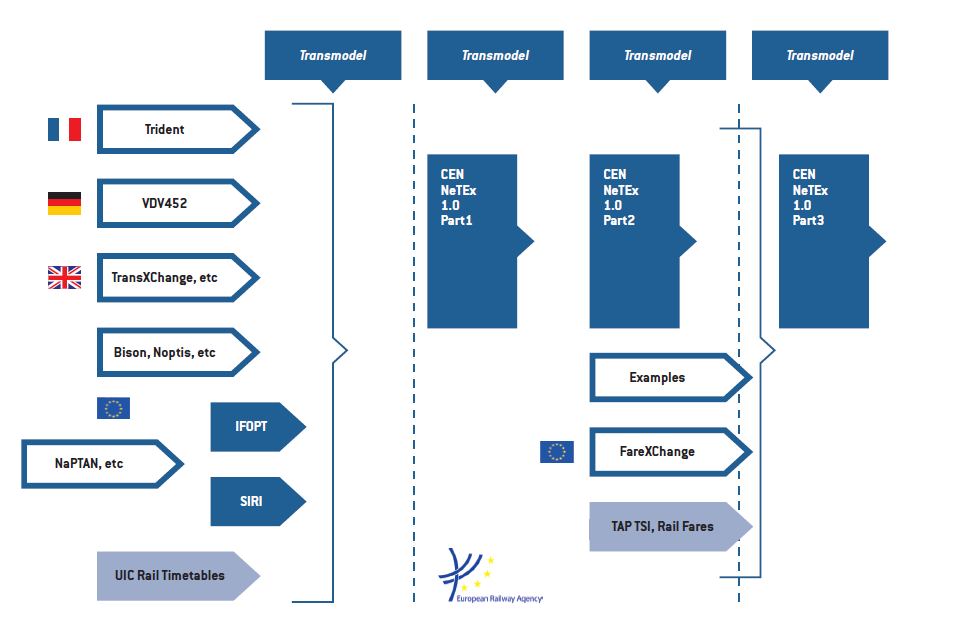
\includegraphics[width=\textwidth]{images/trans.png}
    \caption{Evolution of transmodel, only of the first three parts}
    \label{fig:evolution:transmodel}
\end{figure}
\section*{Reference resolver}
\addcontentsline{toc}{section}{References resolver}
\begin{listing}[H]
\inputminted[frame=single,linenos,breaklines]{TypeScript}{code/resolve_entities.tex}
\caption{Code to create a graph using the references found in an entity.}
\label{code:resolve}
\end{listing}
\section*{Gitlab structure}
\addcontentsline{toc}{section}{Gitlab structure}
The thesis resulted in some Gitlab repo's. A short description of all these repo's you can find below.
\begin{enumerate}
    \item gtfs 2 transmodel ontology
    \item gtfs-downloader
    \item gtfs-serve-large
    \item raptor: This is the
    \item thessis latex: Latex code of the thesis, also contains all images and tikz code.
    \item ts-array-utils: A helper library created by the same author of the raptor implementation. Some changes where made to support newer nodejs versions.
\end{enumerate}

% TODO MAYBE REMOVE THIS
\section*{out of scope}
\addcontentsline{toc}{section}{out of scope} 
\subsection*{SIRI}
SIRI provides an abstract model of common public transport concepts and data structures that enables the exchange of information on transport operations between different computer systems. It was established as a European standard in October 2006 and is a \glsxtrshort{cen} Technical Standard.



\end{appendices}